%!TEX root = thesis.tex

\documentclass[12pt]{article}
\usepackage[spanish,es-noshorthands]{babel}

% Use a new page for each section
\usepackage{titlesec}
\newcommand{\sectionbreak}{\clearpage}

% Margenes
\usepackage{geometry}
\geometry{
  letterpaper,
  top=4cm,
  bottom=3cm,
  left=4cm,
  right=3cm
}

% Fuente
\usepackage{fontspec}
\setmainfont{Times New Roman}

\usepackage[
    backend=biber,
    style=apa,
    doi=true,
    sorting=nyt
]{biblatex}
\addbibresource{biblio.bib}

\usepackage[final]{microtype}
\setlength\emergencystretch{3em} % Emergency margin

% CODE
\usepackage{minted}
\setminted{fontsize=\footnotesize, breaklines, frame=lines}

\renewcommand{\baselinestretch}{1.5}

\newcommand{\ttitle}{Análisis Descriptivo y Predictivo Basado en Datos del Tráfico Vehicular en Antofagasta: Un Enfoque a partir de Reportes de Conductores}
\newcommand{\auth}{Richard Peña Bonifaz}

\usepackage{graphicx}
\usepackage{amsmath}

\usepackage{xurl}
\usepackage{hyperref}
\hypersetup{
    breaklinks=true,
    pdftitle={\ttitle},
    pdfauthor={\auth},
}
\usepackage{float}
\usepackage{parskip}
\usepackage[spanish]{cleveref}

\usepackage{algorithm}
\usepackage{algpseudocode}

\usepackage[caption = true]{subfig}

\usepackage[autostyle]{csquotes}

\begin{document}

\pagenumbering{gobble}

\title{\ttitle}
\author{\auth}
\date{\today}
\maketitle

\section*{Dedicatoria}

A todas las personas que estuvieron conmigo y me alentaron en los momentos más difíciles.

\section*{Reconocimientos}

A los profesores apasionados por su trabajo, que no solo transmiten conocimiento, sino también la pasión por el saber y la aplicación de la materia que imparten.

\newpage
\tableofcontents
\listoffigures
\listoftables
\newpage

\section{Resumen}

\pagenumbering{arabic}
\setcounter{page}{1}

El proyecto desarrollado tuvo como propósito la creación de una herramienta efectiva para analizar y predecir, con alta confiabilidad, el comportamiento del tráfico vehicular en la ciudad de Antofagasta, utilizando datos provenientes de la plataforma Waze Cities. Esta plataforma, alimentada por su comunidad de usuarios, proporciona información en tiempo real que permite obtener una visión detallada de los eventos de tráfico en la ciudad. La investigación resultante generó información relevante para la gestión del tráfico, facilitando la toma de decisiones por parte de las autoridades locales, con miras a mejorar la seguridad vial y optimizar la eficiencia del flujo vehicular. A partir del análisis y explotación de estos datos, fue posible identificar patrones y tendencias que, al ser integrados en la planificación urbana, permiten optimizar rutas críticas, reducir la congestión y disminuir la probabilidad de accidentes.

Se utilizó el algoritmo \texttt{GridSearchCV} para seleccionar los mejores parámetros del modelo acorde a su curva ROC-AUC final. Se probaron tres modelos de clasificación: RandomForestClassifier, LogisticRegression y XGBBoost, siendo este último el modelo seleccionado debido a que obtuvo el mayor rendimiento, con un F1-score de 78.6\% y volumen bajo la curva ROC (ROC-AUC) de 84.3\%. Se utilizaron 52,672 datos para el entrenamiento, 26,336 datos de eventos reportados por conductores (luego de ser filtrados) y 26,336 datos generados de forma ficticia como no-ocurrencia de eventos para el balanceo de clases, debido a la naturaleza de los datos al contener solo registros de ocurrencias.

\section{Introducción}
\subsection{Descripción del problema}

Antofagasta, una ciudad con más de 106,000 vehículos en circulación \parencite{conaset2023}, enfrenta desafíos significativos en la gestión de su tráfico vehicular. Durante el año 2023, se registraron 1,715 accidentes, los cuales resultaron en 31 fallecidos y 102 heridos graves \parencite{conaset2023}. Tuvo un crecimiento de su parque automotor de 0.8\% y 3.5\% en los años 2022 y 2023 respectivamente según datos del INE \parencite{ine2023}.

La infraestructura vial limitada cuenta con dos arterias principales para poder atravesar la ciudad, la Avenida Edmundo Perez Zujovic y la Avenida Pedro Aguirre Cerda, La segunda solo presente en un una parte del recorrido, por lo que para el resto, se deben utilizar diferentes alternativas en similares alturas de la ciudad, ninguna de estas continuas. Esto posiciona a la Avenida Edmundo Perez Zujovic, la cual en el sector sur de la ciudad se encuentra con Avenida Grecia y Avenida Ejército, como la única vía continua que atraviesa la ciudad completamente. Esta particularidad dada las características geográficas de Antofagasta sumada a la alta concentración de vehículos, genera una alta congestión y  riesgo de accidentes, especialmente en las zonas anteriormente mencionadas.

Actualmente, no existe algún sistema de monitoreo en tiempo real que permitan gestionar el tráfico de manera proactiva. Los sistemas de monitoreo tradicionales, como son la gestión de semáforos y el estudio de vías, es valioso para la administración del flujo vehicular y la estandarización de las intersecciones. Sin embargo, tiene limitaciones por ser estático para la vía en donde el diseño fue realizado. Este tipo de gestión tiene la limitación de no permitir una visión global del flujo vehicular, como también la poca flexibilidad ante los cambios que se generan en el entorno \parencite{auld2009}.

Explorar nuevas fuentes de datos, como los eventos vehiculares en la ciudad, o la gestión a través de visión por computadora, son herramientas que permiten gestionar de forma eficiente y efectiva el flujo vehicular, proporcionando datos en tiempo real, también ofrecen opciones de automatización y predictibilidad \parencite{chen2015}. Contar con grandes volúmenes de datos permite desarrollar modelos inteligentes para la gestión del tráfico vehicular.

Waze recopila datos de eventos reportados por los usuarios, los cuales cuentan con tres aspectos principales; el tiempo, la ubicación, y el tipo de evento. Esta categorización permite poder desarrollar modelos que detecten patrones y puedan estimar la probabilidad de eventos futuros, basándose en datos del pasado. Esta opción entrega una visión global de la ciudad, para poder detectar focos de atención en cuanto a la ocurrencia de accidentes y congestión vehicular. El uso de datos colaborativos, como los reportados por usuarios en Waze, ha demostrado ser una fuente válida para el análisis y predicción de patrones de tráfico urbano, permitiendo detectar focos críticos de congestión y accidentes \parencite{ferreira2017waze}.

La plataforma Waze Cities, permite a ciudades poder obtener datos para gestionar el tráfico vehicular con herramientas inteligentes, esto conlleva a mejorar la seguridad y la eficiencia en el tráfico vehicular, usando una fuente de dato ya existente \parencite{wazecitiescasestudies2024}.

\subsection{Metodología}

Se realiza un análisis geoespacial con el objetivo de identificar puntos críticos, como vías principales, calles secundarias y zonas de alto tráfico. Este análisis se llevó a cabo utilizando \texttt{GeoPandas}. Los resultados se presentan mediante técnicas de visualización que permitien interpretar las tendencias y puntos de interés de manera efectiva.

El pipeline de datos incluye una base de datos relacional para almacenarlos, un flujo ETL (Extract, Transform, Load) para procesarlos y un cliente web para visualizarlos. Se utilizó PostgreSQL \parencite{postgres2025} como base de datos SQL, Memcached  \parencite{memcached2025} como base de datos de caché, APScheduler para la programación de tareas y Dash \parencite{dash2025} como herramienta de visualización. Este enfoque permitió automatizar el flujo de datos y garantizar la actualización constante de la información.

Para el proceso de entrenamiento del modelo, se llevó a cabo un balanceo de clases, debido a la naturaleza de los datos, solo contiene datos de la ocurrencia de eventos, esto genera sesgos en el modelo y un sobre-ajuste que hace que el modelo tenga un rendimiento disminuido \parencite{he2009learning}.

Adicionalmente, se entrenó un modelo de clasificación para determinar la probabilidad de ocurrencia de accidentes en diferentes puntos de la ciudad. El modelo seleccionado fue XGBoost \parencite{chen2016xgboost}, el cual fue seleccionado utilizando técnicas de validación cruzada y optimización de hiperparámetros \parencite{geron2019hands}. Para la selección de variables se utilizó GridSearchCV \parencite{pedregosa2011scikit, geron2019hands}, una técnica de búsqueda de hiperparámetros que permite encontrar la mejor combinación de variables para el modelo, se compararon modelos de regresión logística, árboles de decisión y XGBoost.

Para la gestión del modelo, en cuanto a su implementación, mantenimiento y actualización, se programó APSCheduler, para ejecutar tareas periódicas que permiten gestionar el ciclo de vida de los modelos de aprendizaje automático, desde su entrenamiento hasta su despliegue en producción y versionado.

El servidor se desarrolló en \texttt{Rust} \parencite{rust2025}, un lenguaje de programación enfocado en la eficiencia y seguridad en el uso de memoria. Se utilizó \texttt{Memcached} para generar un caché de los datos y de esta forma poder servirlos de manera más eficiente y rápida \parencite{fitzpatrick2004memcached}, debido al volumen de datos, se priorizó la unicidad de los mismos, evitando generar copias, para no aumentar el uso de memoria.

Para el procesado de los datos en el cliente —\texttt{Dash}—, se generan múltiples workers que permiten servir la aplicación de forma eficiente, y se utiliza solo una instancia en memoria de los datos, compartida por todos los workers. Para mantener la integridad de los datos, se implementa un \texttt{Mutex} para controlar el acceso de lectura a los mismos desde las tareas asíncronas \parencite{ramalho2015fluent}.

La perspectiva general del flujo de datos se muestra en la \autoref{fig:fuente} y el flujo desde la API de Waze hasta el dashboard se puede observar en la \autoref{fig:wf_dash}

\begin{figure}[H]
    \centering
    \includegraphics[width=0.8\textwidth]{images/fuente_datos.png}
    \caption{Pipeline general de datos}
    \label{fig:fuente}
\end{figure}

\begin{figure}[H]
    \centering
    \includegraphics[width=0.8\textwidth]{images/wf_dash.png}
    \caption{Flujo de información en dashboard}
    \label{fig:wf_dash}
\end{figure}


\subsection{Objetivo general}

Analizar y modelar el comportamiento del tráfico vehicular en Antofagasta mediante datos de la plataforma Waze, con el fin de desarrollar una herramienta predictiva que contribuya a la gestión eficiente y segura del tráfico urbano.

\subsection{Objetivos específicos}

\begin{itemize}
    \item Realizar un análisis descriptivo de los datos recolectados para identificar patrones y tendencias relevantes en el comportamiento del tráfico.
    \item Presentar información visualmente comprensible y útil para la gestión vial, facilitando la implementación de políticas y acciones basadas en datos.
    \item Proponer una herramienta exploratoria para apoyar la toma de decisiones en la gestión vial
\end{itemize}

\subsection{Alcances}

Los datos utilizados corresponden al periodo desde octubre de 2024 hasta abril de 2025, en el sector urbano de la ciudad de Antofagasta, desde la zona norte urbana actual, sector Costa Laguna, hasta la zona sur, salida a camino de la minería, excluyendo el camino a puerto Coloso.

El área de estudio está delimitada por las coordenadas geográficas 23.35°S a 23.65°S de latitud y 70.36°O a 70.45°O de longitud, correspondientes al sistema de referencia EPSG:4326 (WGS84).

\section{Marco teórico}

El tráfico vehicular en entornos urbanos presenta un comportamiento complejo e impredecible, lo que dificulta su gestión eficiente. No obstante, el avance de las tecnologías móviles y la popularidad de aplicaciones como Waze permiten disponer de datos en tiempo real generados por los propios usuarios. Este proyecto se apoya en técnicas de análisis de datos y aprendizaje de máquinas (Machine Learning) para convertir esta información en herramientas útiles para la gestión vial. La utilización de datos geoespaciales, junto con la automatización de los procesos de recolección, análisis y visualización, constituye una solución costo-efectiva para mejorar la planificación del tráfico \parencite{barcelo2005}.

\subsection{Gestión de la seguridad vial}

Existen diferentes estrategias para la gestión vehicular, desde sistemas manuales como la dirección del tránsito por carabineros; o más automatizados, como la gestión inteligente de semáforos. En términos de seguridad, para evitar la ocurrencia de accidentes, resulta conveniente aplicar la jerarquía de control de riesgo (\autoref{fig:jerarquia_riesgos}). Esta busca abordar desde la medida de mayor impacto, hasta la de menor impacto en la exposición al riesgo. Se divide en dos grupos principales, las barreras duras y las barreras blandas (o administrativas). El primer grupo consta de la eliminación del agente de riesgo, la sustitución por uno de menor exposición o medidas ingenieriles, que buscan administrar la exposición con algún rediseño u organización. Las medidas administrativas constan de diferentes estrategias que puedan cambiar el comportamiento, el cuidado o la visibilidad de la exposición, por último, los elementos de protección personal, que buscan mitigar el daño ante algún posible accidente \parencite{niosh2024}.

\begin{figure}[h]
    \centering
    \includegraphics[width=0.8\textwidth]{images/jerarquia_control_riesgo.png}
    \caption{Jerarquía de control de riesgos. Fuente: \textcite{niosh2024}.}
    \label{fig:jerarquia_riesgos}
\end{figure}

La eliminación de la necesidad de transporte, puede ser abordada con estrategias como el fomento del teletrabajo para los puestos que lo permitan, o haciendo que las personas se encuentren más cerca de sus trabajos, eliminando la necesidad de transporte en vehículo. La sustitución se genera fomentando el uso de transporte público, el uso de medios alternativos de transporte, como las bicicletas o el uso compartido de vehículos. Las medidas de ingeniería buscan optimizar el flujo vehicular, puede ser a través del rediseño del plano urbano, el diseño de vehículos más seguros, monitoreo a través de radares, cámaras y GPS, planificación de rutas y nuevas vías de tránsito. Como medidas administrativas se encuentran la educación vial, la señalización y los límites de velocidad. En cuanto a elementos de protección personal, se posiciona el uso de cinturón de seguridad, la instalación de airbags, barreras anti-vuelco y barreras de contención en las vías, entre otras.

\subsection{Indicadores de bondad y ajuste}

Para evaluar la relación entre variables cuantitativas y validar supuestos estadísticos, se utilizaron indicadores clásicos de ajuste y asociación. En particular, se aplicaron pruebas de hipótesis y el coeficiente de correlación de Pearson, herramientas fundamentales en el análisis estadístico inferencial \parencite{devore2011, montgomery2018}.

La \textbf{prueba de hipótesis} permite evaluar si existe suficiente evidencia en los datos para rechazar una afirmación nula sobre una población. En el caso de correlaciones, la hipótesis nula establece que no existe relación lineal entre las variables (\( H_0 : \rho = 0 \)), mientras que la hipótesis alternativa plantea la existencia de una correlación (\( H_1 : \rho \neq 0 \)). El valor-p obtenido indica la probabilidad de observar un estadístico igual o más extremo, bajo el supuesto de que la hipótesis nula es verdadera. Si el valor-p es inferior al nivel de significancia (\( \alpha \)), se rechaza la hipótesis nula \parencite{devore2011}.

El \textbf{coeficiente de correlación de Pearson} (\( r \)) mide la intensidad y dirección de la relación lineal entre dos variables cuantitativas. Su valor varía entre $-1$ y $1$, donde valores cercanos a $1$ indican una correlación positiva fuerte, valores cercanos a $-1$ una correlación negativa fuerte, y valores cercanos a $0$ una relación débil o inexistente. Este indicador viene dado por:

\begin{equation}
r = \frac{\sum_{i=1}^{n}(x_i - \bar{x})(y_i - \bar{y})}{\sqrt{\sum_{i=1}^{n}(x_i - \bar{x})^2 \sum_{i=1}^{n}(y_i - \bar{y})^2}}
\end{equation}

donde \( x_i \) y \( y_i \) representan los valores observados, y \( \bar{x} \) y \( \bar{y} \) sus respectivas medias \parencite{montgomery2018}.

\subsection{Ciencia de datos para el análisis de comportamiento}

Entender el comportamiento del tráfico vehicular, permite desarrollar medidas ingenieriles que disminuyan la probabilidad de accidentes, gestionando diversas variables como la congestión vehicular, los horarios con mayor probabilidad de accidentes y los sectores con mayor frecuencia de accidentes. La ciencia de datos permite, a través del uso de diferentes herramientas estadísticas, predecir con un grado de certeza conocido, la probabilidad de que ocurra un accidente tomando en cuenta variables que puedan ser determinantes para la ocurrencia de los mismos.

Usando datos de eventos pasados, es posible generar modelos que, a partir de una entrada, entreguen una salida determinada según ciertos parámetros, esto se conoce como análisis predictivo. El análisis predictivo consiste en entrenar modelos con datos históricos para anticipar resultados futuros, utilizando distintas técnicas de aprendizaje automático, las cuales pueden clasificarse en aprendizaje supervisado, no supervisado y por refuerzo \parencite{murphy2012machine, geron2019hands, bishop2006pattern}.

En el aprendizaje supervisado, el modelo recibe tanto los datos de entrada como los de salida esperada, lo que le permite aprender patrones y realizar predicciones sobre nuevos datos con base en ese entrenamiento. El aprendizaje no supervisado utiliza datos de entrada, buscando estructuras o patrones en los mismos sin una clasificación específica, dejando la interpretación a cargo del especialista. Finalmente, en el aprendizaje por refuerzo, el modelo recibe una entrada, ejecuta una acción o predicción, y ajusta su comportamiento en función de una retroalimentación positiva o negativa, con el objetivo de maximizar el rendimiento a lo largo del tiempo.

Adicionalmente, los modelos pueden clasificarse según el tipo de salida que generan: modelos de regresión, que entregan valores numéricos continuos, y modelos de clasificación, que asignan las observaciones a una o más categorías previamente definidas. En estos últimos, el resultado se expresa como una distribución de probabilidades, y se considera como salida final la categoría con mayor probabilidad.

En este estudio se empleó un modelo supervisado de clasificación, con el objetivo de estimar la probabilidad de ocurrencia de un accidente, considerando dos posibles resultados: “ocurre” o “no ocurre”.

\subsection{Evaluación de los modelos de Machine Learning}

Para evaluar el rendimiento del modelo se utilizaron métricas ampliamente empleadas en problemas de clasificación binaria, tales como la exactitud (\textit{accuracy}), la precisión (\textit{precision}), la recuperación (\textit{recall}) y la medida F1 (\textit{F1-score}) \parencite{manning2008}. La exactitud representa el porcentaje total de predicciones correctas sobre el total de casos evaluados. La precisión corresponde a la proporción de casos positivos correctamente identificados por el modelo, es decir, el número de verdaderos positivos dividido por el total de predicciones positivas. Por su parte, la recuperación —también conocida como \textit{recall}— mide la capacidad del modelo para identificar correctamente todos los casos positivos reales, dividiendo los verdaderos positivos por el total de casos positivos reales. La medida F1, en tanto, es la media armónica entre precisión y recuperación, y proporciona una visión equilibrada del desempeño del modelo cuando es necesario considerar tanto los errores por omisión como los errores por comisión.

Además, se construyó una matriz de confusión, la cual permite observar el número de aciertos y errores cometidos en cada clase —“ocurre” y “no ocurre”— lo que facilita una evaluación más detallada del comportamiento del modelo. Este análisis es clave para comprender sus limitaciones y fortalezas, especialmente en aplicaciones reales relacionadas con la predicción de accidentes de tránsito.

Las fórmulas utilizadas para el cálculo de estas métricas son las siguientes:

\[
\begin{aligned}
\text{Exactitud (Accuracy)} &= \frac{TP + TN}{TP + TN + FP + FN} \\
\text{Precisión (Precision)} &= \frac{TP}{TP + FP} \\
\text{Recuperación (Recall)} &= \frac{TP}{TP + FN} \\
\text{Medida F1 (F1-score)} &= 2 \cdot \frac{\text{Precisión} \cdot \text{Recuperación}}{\text{Precisión} + \text{Recuperación}}
\end{aligned}
\]

donde \( TP \) son los verdaderos positivos, \( TN \) los verdaderos negativos, \( FP \) los falsos positivos y \( FN \) los falsos negativos.

\subsection{Algoritmos de clasificación: Random Forest, Logistic Regression y XGBoost}

Para abordar problemas de clasificación binaria, como la predicción de ocurrencia o no ocurrencia de eventos de tráfico, se utilizaron algoritmos de aprendizaje supervisado. En particular, se emplearon los métodos \textit{Random Forest}, \textit{Logistic Regression} y \textit{XGBoost}, los cuales han demostrado un alto rendimiento en tareas de clasificación estructurada \parencite{friedman2001elements, chen2016xgboost, hosmer2013applied}.

\textbf{Random Forest} es un algoritmo basado en el principio del ensamblado de modelos, específicamente mediante la construcción de múltiples árboles de decisión. Cada árbol es entrenado sobre una muestra aleatoria del conjunto de datos (con reemplazo), y en cada nodo del árbol se selecciona una subdivisión óptima a partir de un subconjunto aleatorio de características. Esta técnica, conocida como \textit{bagging} (bootstrap aggregating), permite reducir la varianza del modelo y mejorar su capacidad de generalización. La predicción final se obtiene mediante votación mayoritaria entre todos los árboles del conjunto \parencite{breiman2001random}.

\textbf{Logistic Regression} es uno de los modelos estadísticos más utilizados para tareas de clasificación binaria. Se basa en la estimación de la probabilidad de pertenencia a una clase mediante la función logística o sigmoide, que transforma una combinación lineal de las variables predictoras en valores comprendidos entre 0 y 1. Este enfoque permite interpretar los coeficientes del modelo como efectos marginales sobre la probabilidad de ocurrencia del evento, manteniendo una alta interpretabilidad y simplicidad computacional. No obstante, su desempeño puede verse limitado ante relaciones no lineales o interacciones complejas entre las variables \parencite{hosmer2013applied}.

\textbf{XGBoost} (\textit{Extreme Gradient Boosting}) es un algoritmo basado en el método de \textit{boosting}, donde los árboles son construidos de manera secuencial. A diferencia del \textit{bagging}, el \textit{boosting} busca corregir los errores cometidos por los modelos anteriores, ajustando cada nuevo árbol a los residuos del conjunto anterior. XGBoost optimiza una función de pérdida regularizada utilizando técnicas avanzadas como la poda previa, el manejo eficiente de valores faltantes y una implementación paralelizada, lo que lo convierte en uno de los algoritmos más eficientes y precisos en clasificación tabular \parencite{chen2016xgboost}.

Estos algoritmos permiten capturar relaciones tanto lineales como no lineales entre las variables predictoras y la variable objetivo, siendo adecuados para trabajar con datos heterogéneos, como los recopilados desde fuentes de tráfico urbano. En la etapa de desarrollo se aplicaron los modelos para comparar su desempeño predictivo sobre el conjunto de datos estudiado.

\subsection{Análisis geoespacial}

Waze entrega las coordenadas geoespaciales de los eventos de tráfico en el sistema de referencia \textbf{EPSG:4326}. Este sistema corresponde al datum geodésico global \textbf{WGS84 (World Geodetic System 1984)}, ampliamente utilizado en aplicaciones de posicionamiento global (GPS) y cartografía digital \parencite{epsg4326, wgs84_nima}. En EPSG:4326, las coordenadas están expresadas en grados decimales de latitud y longitud, lo cual es adecuado para visualización, pero no para realizar cálculos métricos directos como distancias o áreas.

Para llevar a cabo análisis espaciales cuantitativos sobre los eventos reportados por Waze —incluyendo cálculos de distancia, densidad y agrupación geográfica— fue necesario transformar dichas coordenadas a un sistema proyectado con unidades métricas.

La transformación se realizó utilizando la proyección Transversa de Mercator (Transverse Mercator), en su implementación como zona UTM 19 Sur (EPSG:32719). Esta proyección es conforme y está basada en el elipsoide WGS84, con un meridiano central en $\lambda_0 = -69^\circ$, un factor de escala $k_0 = 0.9996$, y un falso este de $500\,000$ m. Para el hemisferio sur, además, se aplica una corrección vertical de $10\,000\,000$ m a la coordenada norte. Esto se detalla en el Apéndice~\ref{ap:utm}.

Esta transformación se aplicó mediante la función \texttt{to\_crs} de la librería \texttt{GeoPandas}, la cual utiliza internamente la librería \texttt{Pyproj} como interfaz de la librería PROJ \parencite{gdal_proj, pyproj, geopandas}.

La elección de EPSG:32719 permite minimizar la distorsión local, ya que el sistema UTM divide el globo en zonas longitudinales estrechas, optimizando la precisión en cada región. Al ser una proyección conforme y métrica, asegura que las distancias, áreas y densidades calculadas sobre el plano proyectado sean válidas y consistentes con el Sistema Internacional de Unidades \parencite{epsg32719}.

\subsection{Aprendizaje automático}

A medida que la cantidad de datos aumenta, el modelo requiere ser reentrenado para incorporar los nuevos registros y así actualizar sus parámetros. Este proceso de aprendizaje continuo permite que el modelo se adapte a las variaciones que puedan presentarse en los patrones de tráfico vehicular a lo largo del tiempo. Para asegurar esta adaptabilidad, se programó una frecuencia de reentrenamiento mensual, lo que implica la incorporación de aproximadamente 9,244 nuevos datos al modelo cada mes. El reentrenamiento periódico resulta fundamental para mantener la vigencia y precisión del modelo, ya que permite integrar las tendencias más recientes y responder oportunamente a los cambios en las condiciones del tráfico \parencite{gama2014concept}.


Para la gestión de los modelos se utilizó \texttt{MLFlow}, un \texttt{framework} que permite gestionar las versiones de los modelos y almacenarlos en una base de datos, asegurando la persistencia de los mismos. También permite almacenar las diferentes métricas de cada versión del modelo \parencite{mlflow2025}.

Para la gestión del modelo, en cuanto a su implementación, mantenimiento y actualización, se programó con \texttt{APSCheduler}, una librería de tareas asíncronas en Python \parencite{apscheduler2025}.

\subsection{Investigaciones previas}

El análisis del tráfico vehicular y la predicción de accidentes han sido objeto de múltiples estudios en los últimos años. Por ejemplo, \parencite{barcelo2005} exploraron simulaciones dinámicas de redes de tráfico utilizando AIMSUN, destacando su capacidad para modelar escenarios urbanos complejos. Por otro lado, \parencite{vanlint2005} desarrollaron modelos basados en redes neuronales para predecir tiempos de viaje en autopistas, incluso en condiciones de datos faltantes, demostrando la utilidad de enfoques basados en aprendizaje automático.

En el ámbito de la gestión de tráfico basada en datos, \parencite{chen2015} propusieron enfoques impulsados por datos para la predicción y gestión del tráfico, enfatizando la importancia de integrar fuentes de datos en tiempo real. Asimismo, \parencite{goedertier2009robust} introdujeron técnicas para descubrir procesos robustos mediante eventos negativos artificiales, lo que permite abordar problemas de clasificación supervisada en contextos de tráfico.

Más recientemente, \parencite{berhanu2024} aplicaron aprendizaje automático y análisis espacial para predecir accidentes de tráfico y optimizar rutas en redes urbanas congestionadas, destacando la relevancia de combinar modelos predictivos con análisis geoespacial.

\section{Desarrollo}

Se diseña una estrategia de recolección de datos que garantiza información con un nivel de certeza conocido. La API de Waze Cities, que proporciona información en tiempo real sobre eventos activos, fue la fuente principal de datos. Para lograr un volumen de datos representativo, se implementó un servidor encargado de recopilar y almacenar esta información de manera continua. El servidor fue desarrollado en \texttt{Rust}, utilizando la librería reqwest \parencite{reqwest2025} para extraer los datos desde la API de Waze Cities. Se recolectan los eventos de tráfico y se almacenan en una base de datos PostgreSQL. Este servidor se ejecuta de manera continua actualizando la información cada 2 minutos. La estructura de la base de datos se muestra en la \autoref{fig:db_diagram}.

\begin{figure}[H]
    \centering
    \includegraphics[width=0.8\textwidth]{images/db_diagram.png}
    \caption{Diagrama de la base de datos}
    \label{fig:db_diagram}
\end{figure}

Existen dos estructuras principales, las alertas (\texttt{alerts}) y las congestiones (\texttt{jams}), el primero registra todos los eventos reportados por usuarios, tales como peligros, accidentes, congestión o rutas cerradas. En el caso de los eventos de congestión, son datos generados automáticamente por Waze, los cuales usando la geolocalización, estiman congestiones en diferentes puntos de la ciudad. Para este proyecto, se utiliza la información de las alertas. Sin embargo, se almacenaron los datos de congestión, para un posterior análisis, que está fuera del alcance de este estudio. Esta estructura se definió con base en los datos relevantes y completos que proporciona la API, los tipos de datos disponibles pueden ser consultados en la documentación de Waze \parencite{waze2024}.

Desde octubre de 2024 hasta abril de 2025, se capturan 53,159 alertas, que al ser filtradas (ver \autoref{ssec:filter}), finalmente se obtienen 26,336, las cuales se analizarán a lo largo de este estudio.


\subsection{Filtrado temporal y agrupación de eventos} \label{ssec:filter}

Las alertas pueden contener duplicados, debido a que diferentes usuarios pueden reportar el mismo evento. Para evitar esto, se filtraron los datos agrupándolos por segmento (\autoref{ssec:freq_zone}) y periodos de tiempo, eliminando grupos duplicados en una ventana de tiempo de 120 minutos, es decir, todo evento que se reportó con el mismo tipo, en el mismo segmento, dentro de un periodo de dos horas, será considerado como un solo evento. Este procedimiento, resumido en el \autoref{alg:filter}, permite homogeneizar la granularidad temporal de los eventos y asegurar la consistencia tipológica de los atributos (\texttt{group}, \texttt{type}). El código fuente completo se presenta en el Apéndice~\ref{annex:filter_code}.

De este modo, el filtro actúa como un mecanismo de depuración de ruido observacional, preservando un único registro representativo por evento real. Aunque esta consolidación produce una ligera disminución en las métricas de desempeño (\texttt{ROC AUC} y \texttt{F1-score}), el efecto se considera metodológicamente favorable, ya que aumenta la consistencia temporal y evita el sesgo hacia zonas con mayor densidad de usuarios o reportes. En consecuencia, el modelo resultante refleja con mayor precisión la ocurrencia efectiva de incidentes de tráfico, en lugar de su frecuencia de reporte.


\begin{algorithm}[H]
\caption{Filtrado temporal y agrupación de eventos}
\label{alg:filter}
\begin{algorithmic}[1]
\Require Conjunto de datos $D$, tamaño de intervalo $\Delta t$ (en minutos)
\Ensure Conjunto filtrado y agrupado $D'$

\State $D' \gets \emptyset$
\If{$D = \emptyset$ \textbf{or} no existe columna \texttt{pub\_millis}}
    \State \Return $D'$
\EndIf

\State $D' \gets$ Copia de $D$
\State $paso \gets \Delta t \times 60000$ \Comment{Conversión de minutos a milisegundos}

\ForAll{evento $\in D'$}
    \If{\texttt{pub\_millis} no es entero}
        \State evento.\texttt{pub\_millis} $\gets$ Redondear(evento.\texttt{pub\_millis} / $10^6$)
    \EndIf
    \State evento.\texttt{interval\_start} $\gets \lfloor$evento.\texttt{pub\_millis} / paso$\rfloor \times$ paso
\EndFor

\State Convertir \texttt{interval\_start} a formato fecha-hora (UTC)
\State Asegurar tipo entero en \texttt{group} y tipo texto en \texttt{type}
\State Eliminar duplicados en [\texttt{interval\_start}, \texttt{group}, \texttt{type}]
\State Eliminar columna auxiliar \texttt{interval\_start}
\State Convertir \texttt{pub\_millis} a formato fecha-hora (zona local)
\State Reiniciar índices de $D'$
\State \Return $D'$
\end{algorithmic}
\end{algorithm}


\subsection{Eventos en el espacio y tiempo}

En la \autoref{fig:dist_events} se observa la distribución espacial de los distintos tipos de eventos en la ciudad. Se aprecia una mayor concentración en las principales avenidas, especialmente en el caso de los accidentes, los cuales tienden a ocurrir con mayor frecuencia en los cruces de estas arterias.

\begin{figure}[H]
    \centering
    \subfloat[Accidentes]{
        \includegraphics[width=0.33\textwidth]{images/dist_accidents.png}
    }
    \subfloat[Congestión]{
        \includegraphics[width=0.33\textwidth]{images/dist_jams.png}
    }
    \subfloat[Peligros]{
        \includegraphics[width=0.33\textwidth]{images/dist_hazards.png}
    }
    \caption{Distribución espacial de eventos en Antofagasta}
    \label{fig:dist_events}
\end{figure}

Para el análisis temporal, los eventos se agruparon por hora del día, calculando el promedio de eventos ocurridos por jornada. En la \autoref{fig:time_events} se evidencia una concentración de accidentes y congestiones durante las horas punta. En contraste, los eventos de tipo \texttt{peligro} presentan una distribución más uniforme a lo largo del día.

\begin{figure}[H]
    \centering
    \subfloat[Accidentes]{
        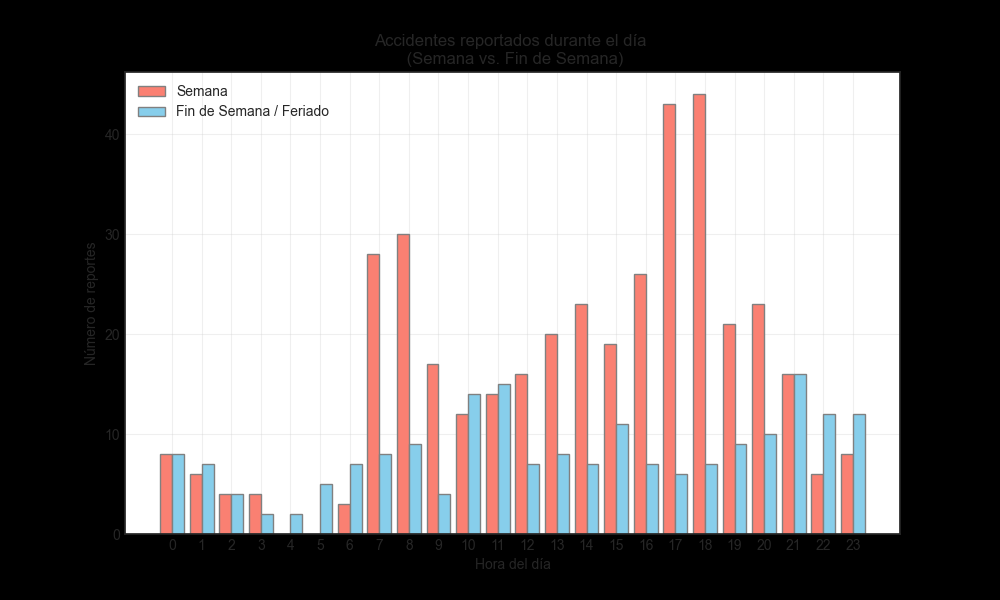
\includegraphics[width=0.6\textwidth]{images/ACCIDENT_per_hour.png}
    }
    \newline
    \subfloat[Congestión]{
        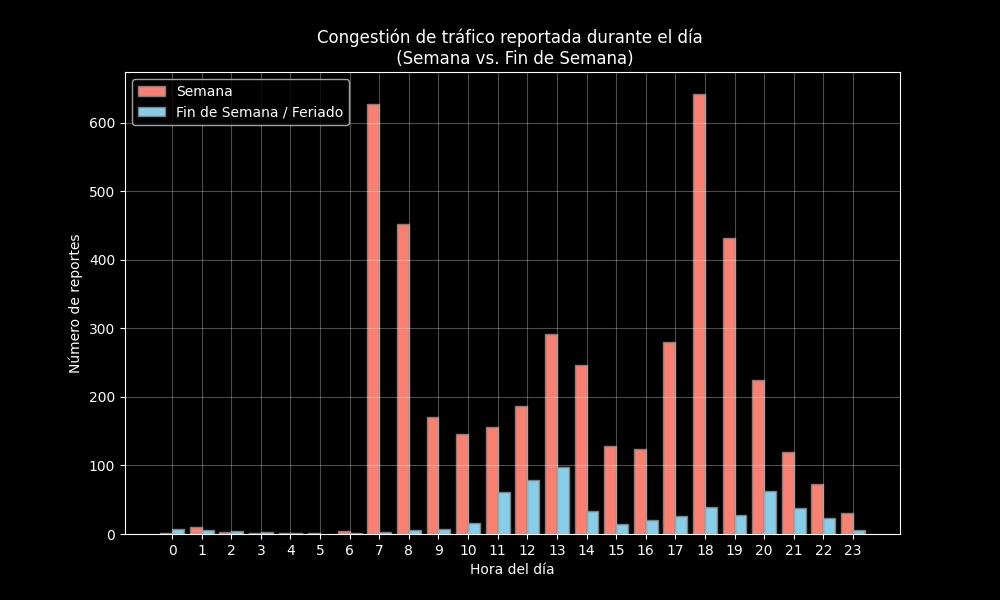
\includegraphics[width=0.6\textwidth]{images/JAM_per_hour.png}
    }
    \newline
    \subfloat[Peligros]{
        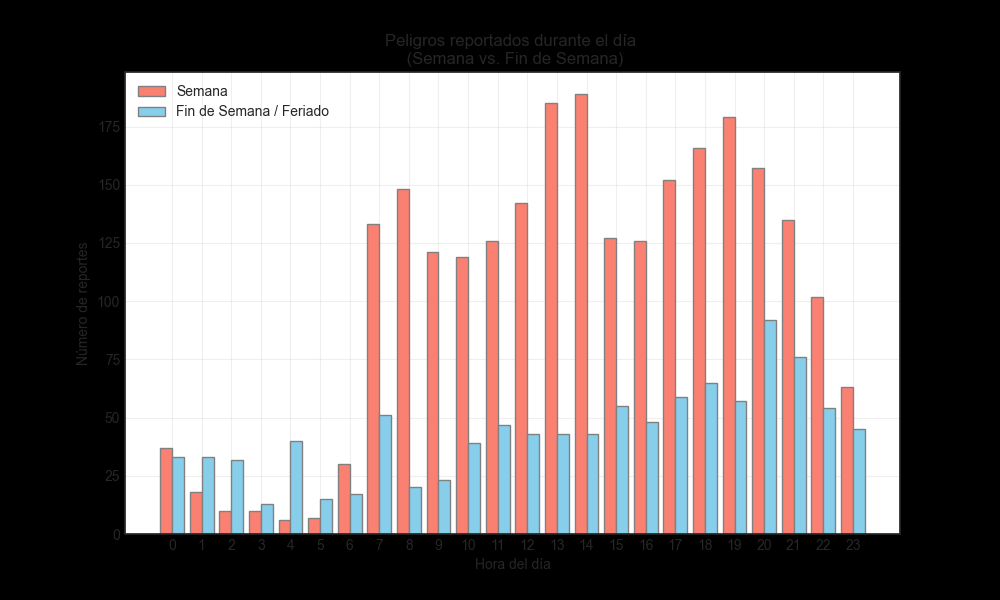
\includegraphics[width=0.6\textwidth]{images/HAZARD_per_hour.png}
    }
    \newline
    \caption{Eventos según hora del día en Antofagasta}
    \label{fig:time_events}
\end{figure}

\subsection{Modelo de correlación lineal}

Los resultados de la regresión lineal entre accidentes y reportes de congestión, presentados en la \autoref{fig:corr_lineal}, indican una fuerte correlación positiva durante los días de semana ($R^2 = 0.90$), lo que no implica necesariamente una causalidad. En cambio, durante los fines de semana la relación es más débil ($R^2 = 0.67$), aunque aún presente.

% Prueba hipótesis relación accidents-jams

\begin{figure}[H]
    \centering
    \subfloat[Día de semana]{
        \includegraphics[width=0.9\textwidth]{images/corr_lin_ds.png}
    }
    \newline
    \subfloat[Fin de semana]{
        \includegraphics[width=0.9\textwidth]{images/corr_lin_fs.png}
    }
    \newline
    \caption{Correlación lineal entre accidentes y congestión}
    \label{fig:corr_lineal}
\end{figure}

\subsection{Prueba de hipótesis de correlación lineal}

Para evaluar la existencia de una relación estadísticamente significativa entre el número de reportes de congestión y la cantidad de accidentes por hora, se aplicó una prueba de correlación de Pearson.

La hipótesis nula ($H_0$) establece que no existe correlación lineal entre ambas variables, mientras que la hipótesis alternativa ($H_1$) plantea que sí existe tal correlación:

\begin{align}
H_0&:\ \rho = 0 \\
H_1&:\ \rho \ne 0
\end{align}

Donde $\rho$ representa el coeficiente de correlación poblacional. El estadístico de prueba se calcula mediante:

\begin{equation}
t = \frac{r \sqrt{n - 2}}{\sqrt{1 - r^2}}
\end{equation}

donde $r$ es el coeficiente de correlación muestral y $n$ el número de observaciones. El valor resultante se contrasta con la distribución t de Student con $n - 2$ grados de libertad.

El análisis estadístico del modelo lineal entregó los siguientes resultados:

\begin{itemize}
    \item Para días de semana:
    \begin{itemize}
        \item El modelo ajustado fue $y = 0.1673x + 0.0996$
        \item Se obtuvo un $R^2 = 0.90$
        \item La significancia global fue $F(1, 22) = 203.33$, $p < 0.0001$
        \item Los parámetros fueron estadísticamente significativos con $p < 0.001$
        \item El estadístico $t$ para la prueba de correlación fue $t = 14.26$, $p < 0.0001$
    \end{itemize}

    \item Para fines de semana:
    \begin{itemize}
        \item El modelo ajustado fue $y = 0.1365x + 0.0748$
        \item Se obtuvo un $R^2 = 0.67$
        \item El coeficiente de correlación de Pearson fue $r = 0.82$ con IC 95\%: [0.62, 0.92]
        \item La significancia global fue $F(1, 22) = 44.42$, $p < 0.0001$
        \item Los parámetros fueron estadísticamente significativos con $p < 0.0001$
        \item El estadístico $t$ para la prueba de correlación fue $t = 6.66$, $p < 0.0001$
    \end{itemize}
\end{itemize}

Estos resultados permiten rechazar la hipótesis nula con un nivel de confianza del 99\% para los días de semana, confirmando la existencia de una relación lineal estadísticamente significativa entre el número de reportes de congestión y la cantidad de accidentes registrados por hora.

Los gráficos Q-Q (\autoref{fig:qq_lin}) muestran una aproximación razonable a la distribución normal en ambos períodos. Para los días de semana, los puntos siguen la línea de referencia, con algunas desviaciones en los extremos, particularmente en los valores más altos. En el caso de fin de semana, la aproximación a la línea teórica es más consistente, con una distribución más cercana a la normal.

Los gráficos de residuos (\autoref{fig:resid_lin}) revelan patrones distintos para cada período. En días de semana, aunque hay cierta dispersión alrededor de cero, se observa variabilidad considerable con algunos residuos positivos destacados (especialmente entre valores ajustados de 0.5 y 0.6) y residuos negativos pronunciados alrededor de 0.8. Para fines de semana, los residuos muestran menor magnitud global, pero un patrón menos aleatorio, sugiriendo posible estructura no capturada por el modelo lineal.

En resumen, el análisis confirma una relación lineal significativa entre congestión y accidentes, considerablemente más fuerte durante días laborables ($R^2 = 0.90$) que en fines de semana ($R^2 = 0.67$). Los patrones observados en los residuos, particularmente para fines de semana, sugieren la pertinencia de explorar modelos no lineales que podrían capturar mejor las relaciones subyacentes en los datos.


\begin{figure}[H]
\centering
\includegraphics[width=0.9\textwidth]{images/residuos_lin.png}
\caption{Residuos del modelo lineal para días de semana y fines de semana}
\label{fig:resid_lin}
\end{figure}

\begin{figure}[H]
\centering
\includegraphics[width=0.9\textwidth]{images/qq_lin.png}
\caption{Gráficos Q-Q de los residuos del modelo lineal}
\label{fig:qq_lin}
\end{figure}


\subsection{Modelo de correlación exponencial inversa}

Dado que la relación entre congestión y accidentes no necesariamente es lineal en todos los contextos —especialmente bajo alta densidad vehicular— se propuso un modelo exponencial inverso.

El modelo propuesto se ajusta a la siguiente forma funcional:

\begin{equation}
A(x) = \frac{\alpha}{x^{\beta}} + \gamma
\end{equation}

donde:
\begin{itemize}
    \item $A(x)$ es el número estimado de accidentes por hora,
    \item $x$ representa el número de reportes de congestión por hora,
    \item $\alpha$, $\beta$ y $\gamma$ son parámetros ajustados mediante regresión no lineal.
\end{itemize}

Este modelo fue aplicado tanto a los días de semana como a los fines de semana. En ambos casos, se observó un ajuste visual considerable, respaldando la hipótesis de una relación decreciente no lineal entre ambas variables bajo ciertas condiciones de tráfico.

Los resultados del ajuste se presentan en la \autoref{fig:corr_exp}, mostrando un ajuste significativo del modelo a los datos.

\begin{figure}[H]
    \centering
    \subfloat[Día de semana]{
        \includegraphics[width=0.9\textwidth]{images/corr_exp_ds.png}
    }
    \newline
    \subfloat[Fin de semana]{
        \includegraphics[width=0.9\textwidth]{images/corr_exp_fs.png}
    }
    \newline
    \caption{Correlación exponencial inversa entre accidentes y congestión}
    \label{fig:corr_exp}
\end{figure}

El análisis estadístico del modelo exponencial inverso entregó resultados significativos tanto para días de semana como para fin de semana:

\begin{itemize}
    \item Para días de semana:
    \begin{itemize}
        \item El modelo ajustado fue $y = 0.3119/x^{-0.6319}$
        \item Se obtuvo un $R^2 = 0.94$
        \item La significancia global fue $F(2, 22) = 158.81$, $p < 0.0001$
        \item Los parámetros fueron estadísticamente significativos con $p < 0.0001$
    \end{itemize}

    \item Para fines de semana:
    \begin{itemize}
        \item El modelo ajustado fue $y = 0.1826/x^{-0.2776}$
        \item Se obtuvo un $R^2 = 0.71$
        \item La significancia global fue $F(2, 22) = 27.19$, $p < 0.001$
        \item Los parámetros fueron estadísticamente significativos con $p < 0.001$
    \end{itemize}
\end{itemize}

Este análisis revela diferencias importantes en la dinámica de la relación congestión-accidentes entre períodos. Durante los días de semana, el exponente negativo de mayor magnitud ($-0.6319$) indica una relación más sensible entre las variables, mientras que en fines de semana el exponente menor ($-0.2776$) sugiere una relación menos pronunciada.

Los gráficos de residuos (\autoref{fig:resid_exp}) muestran una dispersión relativamente aleatoria en torno a cero, sin evidencias claras de heterocedasticidad ni patrones sistemáticos, lo que respalda la validez del ajuste no lineal propuesto. En particular, para los días de semana, los residuos muestran una distribución uniforme con algunos valores extremos (entre -0.1 y 0.2), mientras que para los fines de semana, la dispersión es menor y más equilibrada (aproximadamente entre -0.05 y 0.05).

Complementariamente, los gráficos Q-Q (\autoref{fig:qq_exp}) revelan una aproximación a la distribución normal de los residuos en ambos casos, aunque con algunas desviaciones. En días de semana, se observan algunas desviaciones en los valores extremos, particularmente un punto notable en el extremo positivo. Para los fines de semana, la alineación con la línea teórica es excepcional, indicando una distribución muy cercana a la normal.

En conjunto, estos resultados indican que el modelo exponencial inverso no solo es estadísticamente significativo, sino que además presenta un mejor ajuste que el modelo lineal, especialmente para días de semana donde alcanza un $R^2 = 0.94$ comparado con el $R^2 = 0.90$ del modelo lineal. La normalidad de los residuos y su distribución aleatoria fortalecen la hipótesis de que existe una relación no lineal entre la congestión y la probabilidad de accidentes en contextos urbanos, que puede ser modelada adecuadamente mediante una función exponencial inversa.


\begin{figure}[H]
\centering
\includegraphics[width=0.9\textwidth]{images/residuos_exp.png}
\caption{Residuos del modelo de exponencial inverso para días de semana y fines de semana}
\label{fig:resid_exp}
\end{figure}

\begin{figure}[H]
\centering
\includegraphics[width=0.9\textwidth]{images/qq_exp.png}
\caption{Gráficos Q-Q de los residuos del modelo exponencial inverso}
\label{fig:qq_exp}
\end{figure}

% Cálculo de la frecuencia por zona
% Filtro por zona
%    Algóritmo cKDTree

\subsection{Frecuencia por zona} \label{ssec:freq_zone}

Para representar conjuntos estáticos de puntos espaciales, se utiliza la estructura Kd-tree que computa distancias relativas mediante spiral codes y las almacena usando Directly Addressable Codes (DACs), optimizando el uso de memoria sin sacrificar eficiencia en consultas espaciales \parencite{gutierrez2023ckdtree}. Cada zona es llamada cuadrante o segmento.

En la \autoref{fig:quad_acc} se puede ver cómo se distribuyen los segmentos numéricamente, comenzando desde el segmento 1 en la esquina inferior izquierda. La opacidad del color rojo está relacionada con la cantidad de accidentes por segmento.

\begin{figure}[H]
    \centering
    \includegraphics[width=0.38\textwidth]{images/quad_acc.png}
    \caption{Identificación de cuadrantes en mapa de Antofagasta}
    \label{fig:quad_acc}
\end{figure}

Considerando la media de accidentes diarios, se agrupa por segmento, se define que las zonas mayores a 0.5 accidentes por día son considerados críticos, se construye un mapa según la criticidad (\autoref{fig:quad_mean_day}), al tomar la suma de los accidentes, se obtiene la \autoref{fig:quad_acc_total} que muestra la cantidad de accidentes reportados en el segmento en el periodo de estudio, que a su vez se clasifican como críticos si poseen más de 90 accidentes.

\begin{figure}[H]
    \centering
    \subfloat[Media de accidentes por día]{
        \includegraphics[width=0.4\textwidth]{images/quad_mean_day_color.png}
        \label{fig:quad_mean_day}
    }
    \subfloat[Total accidentes]{
        \includegraphics[width=0.4\textwidth]{images/quad_acc_color.png}
        \label{fig:quad_acc_total}
    }
    \caption{Accidentes por segmento}
\end{figure}

\subsection{Selección del modelo de Machine Learning}

%
% # RandomForest
% rf = RandomForestClassifier(random_state=RANDOM_STATE, n_jobs=-1)
% rf_grid = {
%     "n_estimators": [200, 350, 500],
%     "max_depth": [None, 10, 20],
%     "min_samples_leaf": [1, 3],
%     "class_weight": [None, "balanced"],
% }
%
% [RandomForest] best CV ROC-AUC: 0.8414
% [RandomForest] best params: {'class_weight': None, 'max_depth': 20, 'min_samples_leaf': 3, 'n_estima
% tors': 500}
%
% # LogisticRegression (with scaling in a Pipeline)
% lr_pipeline = Pipeline([
%     ("scaler", StandardScaler(with_mean=False)),  # with_mean=False keeps sparse safety if present
%     ("clf", LogisticRegression(max_iter=2000, random_state=RANDOM_STATE)),
% ])
%
% [LogisticRegression] best CV ROC-AUC: 0.7566
% [LogisticRegression] best params: {'clf__C': 0.1, 'clf__class_weight': 'balanced', 'clf__penalty': '
% l2', 'clf__solver': 'lbfgs'}
%
% # XGBClassifier
% xgb = XGBClassifier(
%     random_state=RANDOM_STATE,
%     n_estimators=400,
%     objective="binary:logistic",
%     tree_method="hist",
%     eval_metric="auc",
%     n_jobs=-1,
% )
% xgb_grid = {
%     "max_depth": [3, 6, 10, 20],
%     "n_estimators": [80, 100],
%     "learning_rate": [0.1, 0.03],
%     "gamma": [0.8, 1.0],
%     "subsample": [0.8, 1.0],
%     "colsample_bytree": [0.8, 1.0],
%     "min_child_weight": [1, 3],
% }
%
% [XGBoost] best CV ROC-AUC: 0.8480
% [XGBoost] best params: {'colsample_bytree': 0.8, 'gamma': 1.0, 'learning_rate': 0.1, 'max_depth': 10
% , 'min_child_weight': 1, 'n_estimators': 80, 'subsample': 0.8}
%
%
%                 model  accuracy  precision    recall        f1   roc_auc    pr_auc
% 0             XGBoost  0.771112   0.738636  0.839156  0.785694  0.843327  0.810811
% 1        RandomForest  0.766935   0.734552  0.835966  0.781985  0.839358  0.807292
% 2  LogisticRegression  0.717269   0.672954  0.845383  0.749377  0.746327  0.659040
%
% RandomForest — Confusion Matrix
% [[4595 1989]
%  [1080 5504]]
% TN=4595, FP=1989, FN=1080, TP=5504
%
% LogisticRegression — Confusion Matrix
% [[3879 2705]
%  [1018 5566]]
% TN=3879, FP=2705, FN=1018, TP=5566
%
% XGBoost — Confusion Matrix
% [[4629 1955]
%  [1059 5525]]
% TN=4629, FP=1955, FN=1059, TP=5525
%

Se evaluaron tres modelos de clasificación para seleccionar el con mejor rendimiento, para ello primero se seleccionaron los mejores hiperparámetros para cada uno basado en la \texttt{curva ROC-AUC}, realizando una búsqueda exhaustiva (\textit{GridSearchCV}) sobre los tres modelos: \textbf{Random Forest}, \textbf{Logistic Regression} y \textbf{XGBoost}.

\paragraph{Random Forest.}
Se evaluaron los siguientes hiperparámetros:

\begin{itemize}
    \item \texttt{n\_estimators}: [200, 350, 500]
    \item \texttt{max\_depth}: [None, 10, 20]
    \item \texttt{min\_samples\_leaf}: [1, 3]
    \item \texttt{class\_weight}: [None, 'balanced']
\end{itemize}

Los mejores hiperparámetros obtenidos fueron:

\begin{itemize}
    \item \texttt{n\_estimators}: 500
    \item \texttt{max\_depth}: 20
    \item \texttt{min\_samples\_leaf}: 3
    \item \texttt{class\_weight}: None
\end{itemize}

Con estos valores, el modelo alcanzó una puntuación máxima de \textbf{0.8414} en validación cruzada (métrica ROC–AUC).

\paragraph{Regresión Logística.}
Se evaluaron los siguientes hiperparámetros:

\begin{itemize}
    \item \texttt{clf\_\_penalty}: [l2]
    \item \texttt{clf\_\_solver}: ['lbfgs', 'liblinear']
    \item \texttt{clf\_\_C}: [0.1, 1.0, 10.0]
    \item \texttt{clf\_\_class\_weight}: [None, 'balanced']
\end{itemize}

Los mejores hiperparámetros obtenidos fueron:

\begin{itemize}
    \item \texttt{clf\_\_penalty}: l2
    \item \texttt{clf\_\_solver}: lbfgs
    \item \texttt{clf\_\_C}: 0.1
    \item \texttt{clf\_\_class\_weight}: balanced
\end{itemize}

El modelo obtuvo una puntuación de \textbf{0.7566} en validación cruzada (ROC–AUC).

\paragraph{XGBoost.}
Se evaluaron los siguientes hiperparámetros:

\begin{itemize}
    \item \texttt{colsample\_bytree}: [0.8, 1.0]
    \item \texttt{gamma}: [0.8, 1.0]
    \item \texttt{learning\_rate}: [0.1, 0.03]
    \item \texttt{max\_depth}: [3, 6, 10, 20]
    \item \texttt{min\_child\_weight}: [1, 3]
    \item \texttt{n\_estimators}: [80, 100]
    \item \texttt{subsample}: [0.8, 1.0]
\end{itemize}

Los mejores hiperparámetros obtenidos fueron:

\begin{itemize}
    \item \texttt{colsample\_bytree}: 0.8
    \item \texttt{gamma}: 1.0
    \item \texttt{learning\_rate}: 0.1
    \item \texttt{max\_depth}: 10
    \item \texttt{min\_child\_weight}: 1
    \item \texttt{n\_estimators}: 80
    \item \texttt{subsample}: 0.8
\end{itemize}

Con estos valores, el modelo XGBoost alcanzó la mejor puntuación promedio en validación cruzada, con un \textbf{ROC–AUC de 0.8480}, confirmando su superior capacidad de generalización frente a los otros modelos.

En el \autoref{tab:model-comparison} se puede observar la comparación de los modelos.

\begin{table}[H]
\centering
\begin{tabular}{|l|p{5.5cm}|c|c|}
\hline
\textbf{Modelo} & \textbf{Mejores Hiperparámetros} & \textbf{ROC AUC} & \textbf{PR AUC} \\
\hline
\textbf{Random Forest} &
\begin{tabular}[c]{@{}l@{}}
\texttt{class\_weight}: None\\
\texttt{max\_depth}: 10\\
\texttt{max\_features}: 2\\
\texttt{max\_leaf\_nodes}: 8\\
\texttt{min\_samples\_leaf}: 2\\
\texttt{n\_estimators}: 100
\end{tabular}
& 0.8394 & 0.8073 \\
\hline
\textbf{XGBoost} &
\begin{tabular}[c]{@{}l@{}}
\texttt{colsample\_bytree}: 0.7\\
\texttt{gamma}: 1\\
\texttt{learning\_rate}: 0.1\\
\texttt{max\_depth}: 30\\
\texttt{n\_estimators}: 80
\end{tabular}
& \textbf{0.8433} & \textbf{0.8108} \\
\hline
\textbf{Regresión Logística} &
\begin{tabular}[c]{@{}l@{}}
\texttt{penalty}: l2\\
\texttt{solver}: lbfgs\\
\texttt{max\_iter}: 1000
\end{tabular}
& 0.7463 & 0.6590 \\
\hline
\end{tabular}
\caption{Comparativa de modelos ajustados con \texttt{GridSearchCV} según el área bajo las curvas ROC y Precision–Recall (PR AUC).}
\label{tab:model-comparison}
\end{table}

Los gráficos de la curva ROC están representados en la \autoref{fig:ROC} y de la curva Precision-Recall en la \autoref{fig:prec-recall}.

\begin{figure}[H]
    \centering
    \includegraphics[width=0.9\textwidth]{images/ROC.png}
    \caption{Curvas ROC}
    \label{fig:ROC}
\end{figure}

\begin{figure}[H]
    \centering
    \includegraphics[width=0.9\textwidth]{images/Precision-Recall.png}
    \caption{Curvas Precision-Recall}
    \label{fig:prec-recall}
\end{figure}

\subsection{Generación de eventos negativos simulados} \label{ssec:class_balancing}

Dado que el conjunto original contiene únicamente eventos positivos (ocurridos), fue necesario generar instancias negativas (no ocurridos) para entrenar un modelo de clasificación binaria. Para ello, se implementó una estrategia inspirada en el enfoque de generación de eventos negativos artificiales propuesto por Goedertier et al. \parencite{goedertier2009robust}, el cual permite representar problemas secuenciales como tareas de clasificación supervisada.

A diferencia del algoritmo original, en el caso del tráfico vehicular se adoptó una relación 1:1 entre eventos positivos y negativos —esto es, se genera un evento negativo por cada evento positivo—, priorizando la eficiencia mediante operaciones vectorizadas y una estructura de datos matricial. Además, debido a que cada evento es independiente de los demás, no se aplicó la noción de causalidad ni las restricciones de paralelismo introducidas por Goedertier, propias de los procesos secuenciales.

En este contexto, la generación de eventos negativos se basa en una grilla temporal con intervalos de 5 minutos, sobre la cual se combinan todas las posibles ubicaciones (\texttt{segmento}) y tipos de evento. Se identifican aquellas combinaciones que no se encuentran en los datos originales —donde no ocurrió un evento— y se etiquetan como eventos negativos (\texttt{happen} = 0). Estas instancias se muestrean aleatoriamente hasta igualar la cantidad de eventos positivos, obteniendo así un conjunto balanceado con un 50\% de instancias positivas y 50\% negativas.

Este enfoque permite preservar la estructura temporal y geoespacial de los datos reales, evitando introducir ruido artificial y facilitando una evaluación más robusta de métricas de desempeño como \texttt{recall} y \texttt{precision}.

El procedimiento se resume en el \autoref{alg:neg_events}. El código completo se incluye en el Apéndice~\ref{annex:neg_code}.

\begin{algorithm}[H]
\caption{Generación de eventos negativos artificiales}
\label{alg:neg_events}
\begin{algorithmic}[1]
\Require Conjunto de eventos positivos $D$, atributo geográfico $g$, tamaño de intervalo $t = 5$ minutos
\Ensure Conjunto balanceado $D'$ con eventos positivos y negativos

\State Convertir marcas de tiempo a milisegundos y definir intervalos temporales de tamaño $t$
\State Agrupar eventos por combinación de $(intervalo, g, tipo)$
\State Generar todas las combinaciones posibles de $(intervalo, g, tipo)$
\State Identificar combinaciones ausentes en $D$ como eventos negativos (\texttt{happen} = 0)
\State Muestrear aleatoriamente los eventos negativos hasta igualar la cantidad de positivos
\State Asignar ubicaciones aleatorias dentro del mismo grupo geográfico $g$
\State Combinar eventos positivos y negativos en un único conjunto balanceado $D'$
\State \Return $D'$
\end{algorithmic}
\end{algorithm}

\subsection{Resultados del modelo seleccionado}

La versión final del modelo (\texttt{v6}) se entrenó utilizando los hiperparámetros obtenidos durante la etapa de validación cruzada. El modelo fue registrado y versionado mediante \textit{MLflow}, permitiendo un seguimiento detallado de sus parámetros y métricas.

El modelo utiliza codificación \textit{one-hot} y un esquema de clasificación binaria (\texttt{binary: logistic}), con una semilla aleatoria (\texttt{random\_state = 42}) para garantizar la reproducibilidad \parencite{geron2019hands}


\noindent En cuanto al rendimiento, se obtuvieron los siguientes resultados para una muestra de 52,672 eventos, con un 50\% de eventos ocurridos y un 50\% de no ocurridos. Esta proporción se logró mediante la simulación de eventos negativos sobre una grilla temporal de 5 minutos, generando combinaciones posibles de tiempo, localización y tipo de evento que no están presentes en los datos originales (\autoref{ssec:class_balancing}). Esto permite evaluar el modelo en condiciones balanceadas, facilitando la interpretación de métricas como \texttt{precision}, \texttt{recall} y \texttt{F1-score}.

\begin{itemize}
    \item \textbf{Accuracy}: 0.8795
    \item \textbf{Recall}: 0.9076
    \item \textbf{Precision}: 0.8583
    \item \textbf{F1-score}: 0.8823
    \item \textbf{Promedio validación cruzada (10 folds)}: 0.7819
\end{itemize}

\noindent Respecto a la matriz de confusión, se registraron los siguientes valores:

\begin{itemize}
    \item Verdaderos positivos: 5,539
    \item Verdaderos negativos: 5,843
    \item Falsos positivos: 965
    \item Falsos negativos: 595
\end{itemize}

Estas métricas evidencian un modelo con gran capacidad para identificar correctamente los casos positivos, sin sacrificar precisión ni equilibrio. La validación cruzada muestra estabilidad a lo largo de los distintos \texttt{folds}, lo que refuerza la robustez del modelo final y confirma que no hubo sobreentrenamiento \parencite{geron2019hands}.

\subsection{Curva de aprendizaje del modelo}

La \autoref{fig:learning_curve} muestra la curva de aprendizaje del modelo XGBoost entrenado. Se observa un rendimiento alto y consistente tanto en el conjunto de entrenamiento como en el de validación (aproximadamente 0.88–0.90), con una brecha mínima entre ambas curvas. Esto indica que el modelo generaliza adecuadamente, sin presentar sobreajuste ni subajuste. Además, el comportamiento plano de ambas curvas sugiere que incrementar el tamaño del conjunto de entrenamiento no tendría un impacto significativo en el rendimiento, lo cual evidencia una saturación en la capacidad de aprendizaje del modelo con las características actuales \parencite{raschka2018,chen2015}.

\begin{figure}[H]
    \centering
    \includegraphics[width=0.8\textwidth]{images/learning_curve.png}
    \caption{Curva de aprendizaje del modelo XGBoost: desempeño en entrenamiento y validación.}
    \label{fig:learning_curve}
\end{figure}

% Aplicación implementación (dashboard online y ML)

\subsection{Despliegue y mantenimiento del modelo}

Para entregar una interfaz que permita al usuario final interactuar con los datos, se desarrolló un tablero de control utilizando \texttt{Dash}, un marco de trabajo especializado en la presentación de datos gráficos mediante Python. La arquitectura del sistema se diseñó siguiendo el patrón cliente-servidor: el servidor implementado en Rust y el cliente en Python, como se muestra en la \autoref{fig:architecture}. El servidor se encarga de las operaciones intensivas como la captura, transformación, almacenamiento y gestión del caché de los datos, mientras que el cliente maneja la interacción con el usuario, la actualización de datos desde el servidor, el entrenamiento del modelo y la generación del tablero de control.

El ciclo de vida del modelo se gestiona mediante APScheduler. Esto permite automatizar el reentrenamiento periódico del modelo con nuevos datos, garantizando su actualización y adaptación a los cambios en los patrones de tráfico.

En el servidor se utiliza Memcached como sistema de caché para optimizar el acceso a los datos frecuentemente consultados, implementando una estrategia de almacenamiento que prioriza la unicidad de los datos para minimizar el uso de memoria. En el lado del cliente, se implementa un sistema de workers múltiples que comparten una única instancia de los datos en memoria, protegida mediante un \texttt{Mutex} para garantizar la integridad en las operaciones de lectura concurrentes.

\begin{figure}[H]
    \centering
    \includegraphics[width=0.8\textwidth]{images/dashboard.png}
    \caption{Arquitectura del sistema}
    \label{fig:architecture}
\end{figure}

El entrenamiento del modelo está programado para realizarse cada 30 días, utilizando los nuevos datos. Los datos del dashboard se actualizan cada 5 minutos.

\section{Discusiones}

\subsection{Patrones espaciales y temporales del tráfico}

El análisis integrado de datos geoespaciales y temporales permitió identificar patrones críticos de siniestralidad en Antofagasta. Destacan como focos principales los segmentos del eje Pedro Aguirre Cerda, especialmente el cruce con Nicolás Tirado (segmentos 106–109), así como la intersección Salvador Allende–Edmundo Pérez Zujovic (segmentos 84 y 103), donde confluyen flujos significativos de vehículos desde distintos sectores de la ciudad. El centro urbano (segmento 82) también presenta una elevada concentración de incidentes.

El análisis temporal evidenció una correlación entre la frecuencia de accidentes y la congestión del tráfico, en línea con la literatura sobre tráfico urbano \parencite{berhanu2024}. Esto sugiere que podría existir una relación de causalidad entre ambas variables, lo cual debe ser evidenciado utilizando métodos adicionales para la investigación.

\subsection{Desempeño y comparación de modelos predictivos}

En la modelación estadística, se observó una correlación significativa entre la congestión reportada y la ocurrencia de accidentes, especialmente en días laborales. El modelo exponencial inverso logró un ajuste superior ($R^2 = 0.96$) respecto al modelo lineal ($R^2 = 0.92$).

El modelo XGBoost logró un desempeño destacado en la predicción de accidentes, con un \textbf{F1-score de 0.88} y un \textbf{Recall de 0.91} en el conjunto de validación. Si bien no se realizó una comparación directa y sistemática con todos los modelos clásicos de series temporales, los resultados obtenidos sugieren que los algoritmos de aprendizaje automático como XGBoost pueden capturar relaciones no lineales y complejas entre las variables predictoras.

El análisis temporal sugiere una mayor frecuencia de accidentes en días hábiles y horarios punta. Se debe contrastar esta relación utilizando nuevas fuentes de información como puede ser la visión por computadora o evaluaciones en terreno \parencite{goodall2019}.

\subsection{Aporte del análisis geoespacial}

El enfoque geoespacial permitió visualizar con claridad zonas críticas y patrones de concentración que no serían evidentes mediante análisis tabulares convencionales. Las visualizaciones generadas, como la \autoref{fig:quad_acc_total} y \autoref{fig:quad_mean_day}, ofrecen una herramienta valiosa para autoridades y planificadores, facilitando la priorización de intervenciones y el diseño de políticas viales focalizadas. Sin embargo, la calidad de estos análisis depende de la completitud y precisión de los datos de referencia, lo cual puede limitar su aplicabilidad en zonas con cartografía incompleta o baja densidad de reportes.

\subsection{Implicancias prácticas y futuras aplicaciones}

El sistema desarrollado evidencia el potencial de los datos colaborativos y el aprendizaje automático para mejorar la gestión del tráfico en ciudades de tamaño medio. Su arquitectura modular y su enfoque basado en datos abiertos facilitan la replicabilidad en otras urbes chilenas. Además, la actualización periódica del modelo y la visualización en tiempo real abren la puerta a su integración con sistemas de gestión vial, aplicaciones móviles o incluso plataformas de respuesta ante emergencias y eventos masivos.

Futuras aplicaciones podrían incluir la incorporación de datos meteorológicos, información de infraestructura o variables de comportamiento humano, así como la exploración de modelos más avanzados (por ejemplo, LSTM o transformers) que capturen mejor la naturaleza secuencial y dinámica del tráfico.

\subsection{Limitaciones del estudio}

El presente trabajo enfrentó diversas restricciones asociadas principalmente a la disponibilidad y calidad de los datos utilizados. Destaca la ausencia de fuentes independientes que permitieran contrastar y validar físicamente los reportes de incidentes, así como la falta de acceso a información relevante sobre la operación de semáforos y las características específicas de los accidentes (por ejemplo, gravedad, causa o participantes involucrados). Esta carencia de datos complementarios limita la posibilidad de validar exhaustivamente los resultados obtenidos. Adicionalmente, no se contó con evidencia en video ni registros visuales que permitieran corroborar la ocurrencia y naturaleza de los eventos reportados.

La generalización de los resultados debe abordarse con cautela, considerando las particularidades urbanas y culturales de cada ciudad, así como las limitaciones del enfoque aplicado. Finalmente, la adopción de modelos complejos puede suponer un desafío adicional en cuanto a la transparencia y comprensión de los resultados por parte de los usuarios finales.

\section{Conclusiones}

Este estudio demuestra la factibilidad y el impacto del uso de datos colaborativos para la gestión inteligente del tráfico urbano en Antofagasta. Los principales aportes incluyen:

\begin{itemize}
    \item Identificación precisa de zonas críticas con alta concentración de accidentes.
    \item Confirmación de una correlación estadísticamente significativa entre congestión y accidentes, especialmente durante días laborales.
    \item Validación de modelos no lineales y de aprendizaje automático como herramientas para la predicción de incidentes en contextos urbanos densos.
    \item Desarrollo e implementación de un sistema funcional de monitoreo, visualización y actualización periódica del modelo, con potencial de escalabilidad.
\end{itemize}

El enfoque propuesto es viable y adaptable, constituyendo una base sólida para futuras iniciativas de movilidad urbana orientadas a la seguridad y eficiencia.

\section{Recomendaciones}

En base a los hallazgos, se sugiere:

\begin{itemize}
    \item \textbf{Intervención focalizada}: Priorizar mejoras de infraestructura, señalización y fiscalización en los segmentos críticos identificados.
    \item \textbf{Monitoreo y actualización}: Mantener y ampliar la infraestructura de captura y análisis de datos, integrando nuevas fuentes (sensores, cámaras) y promoviendo la actualización continua del modelo.
    \item \textbf{Validación cruzada}: Complementar los análisis con estudios de campo y encuestas a usuarios para validar y enriquecer los hallazgos.
    \item \textbf{Escalabilidad}: Replicar y adaptar la metodología a otras ciudades chilenas con características similares, atendiendo a sus particularidades.
    \item \textbf{Investigación avanzada}: Incorporar nuevas variables (clima, infraestructura, comportamiento humano) y explorar modelos predictivos de mayor complejidad y capacidad explicativa.
\end{itemize}

Estas recomendaciones buscan fortalecer una gestión vial proactiva y basada en datos, orientada a la reducción de accidentes y la mejora sostenida de la movilidad urbana.

\newpage

\appendix

\pagenumbering{Alph}
\setcounter{page}{1}

\section{Transformación de coordenadas UTM}
\label{ap:utm}

La proyección UTM utilizada en este estudio (EPSG:32719) se basa en la proyección Transversa de Mercator, adaptada al hemisferio sur y centrada en el meridiano $\lambda_0 = -69^\circ$. Esta proyección es conforme y está diseñada para minimizar la distorsión métrica en una zona longitudinal específica (zona 19S), siendo especialmente adecuada para representar regiones como Antofagasta.

A continuación se presentan las fórmulas que permiten convertir coordenadas geográficas $(\phi, \lambda)$ —latitud y longitud en radianes— a coordenadas planas proyectadas $(x, y)$ en metros, basadas en el elipsoide WGS84:

\subsection*{Parámetros del elipsoide WGS84}

\begin{itemize}
  \item Semieje mayor: $a = 6378137.0$ m
  \item Aplanamiento: $f = \frac{1}{298.257223563}$
  \item Excentricidad: $e^2 = 2f - f^2$
  \item Factor de escala: $k_0 = 0.9996$
  \item Falso este: $E_0 = 500\,000$ m
  \item Falso norte (hemisferio sur): $N_0 = 10\,000\,000$ m
\end{itemize}

\subsection*{Variables intermedias}

\begin{align*}
e'^2 &= \frac{e^2}{1 - e^2} \\
N &= \frac{a}{\sqrt{1 - e^2 \sin^2 \phi}} \\
T &= \tan^2 \phi \\
C &= e'^2 \cos^2 \phi \\
A &= (\lambda - \lambda_0) \cos \phi
\end{align*}

\subsection*{Cálculo del arco meridiano}

\begin{align*}
M &= a \cdot \left[
(1 - \frac{e^2}{4} - \frac{3e^4}{64} - \frac{5e^6}{256}) \phi \right. \\
&\quad - (\frac{3e^2}{8} + \frac{3e^4}{32} + \frac{45e^6}{1024}) \sin(2\phi) \\
&\quad + (\frac{15e^4}{256} + \frac{45e^6}{1024}) \sin(4\phi) \\
&\quad \left. - (\frac{35e^6}{3072}) \sin(6\phi)
\right]
\end{align*}

\subsection*{Coordenadas proyectadas}

\begin{equation}
\begin{split}
y &= N_0 + k_0 \left[ M + N \tan \phi \left( \frac{A^2}{2} \right.\right. \\
&\quad \left.\left. + \frac{A^4}{24}(5 - T + 9C + 4C^2) + \frac{A^6}{720}(61 - 58T + T^2 + 600C - 330e'^2) \right) \right]
\end{split}
\end{equation}

Estas expresiones corresponden a un desarrollo en serie basado en una expansión de Taylor, que permite una transformación precisa desde la superficie curva del elipsoide a un plano cartesiano. Estas fórmulas son utilizadas internamente por la biblioteca PROJ, y fueron documentadas formalmente por Snyder \parencite{snyder1987}.

\subsection*{Nota}

La implementación computacional de estas fórmulas puede realizarse utilizando bibliotecas como \texttt{Pyproj}, que encapsulan estos desarrollos y gestionan automáticamente los parámetros de cada sistema de referencia (CRS).

\section{Código fuente: Filtrado temporal y agrupación de eventos}
\label{annex:filter_code}

\begin{minted}[fontsize=\footnotesize,breaklines,frame=lines]{python}
def filter_by_group_time(self, timedelta_min: int, inplace: bool = False) -> gpd.GeoDataFrame | pd.DataFrame:
    """
    Filter and group data by time intervals.
    """
    if self.data is None or "pub_millis" not in self.data.columns:
        return pd.DataFrame()

    data = self.data.copy() if not inplace else self.data

    if not np.issubdtype(data["pub_millis"].dtype, np.integer):
        data["pub_millis"] = round(data["pub_millis"].astype(np.int64, errors="ignore") / 1_000_000).astype(np.int64)

    step = np.int64(60_000 * timedelta_min)
    data["interval_start"] = ((data["pub_millis"]).to_numpy() // step) * step

    data["interval_start"] = pd.to_datetime(data["interval_start"], unit="ms", utc=True)
    data["interval_start"] = data["interval_start"].dt.tz_convert(utils.TZ)

    data["group"] = data["group"].astype(np.int16)
    data["type"] = data["type"].astype(str)

    data.drop_duplicates(subset=["interval_start", "group", "type"], inplace=True)
    data.drop(columns=["interval_start"], inplace=True)

    if not pd.api.types.is_datetime64_any_dtype(data["pub_millis"]):
        data["pub_millis"] = pd.to_datetime(data["pub_millis"], unit="ms", utc=True)
        data["pub_millis"] = data["pub_millis"].dt.tz_convert(utils.TZ)

    data.reset_index(drop=True, inplace=True)
    return data
\end{minted}

Código: \\
\url{https://github.com/richardhapb/antof-traffic-client/blob/72c1e2cea730670bffb58f0844cd71d1888481df/src/analytics/alerts.py#L100}

\noindent\textbf{Nota:}
La función utiliza la zona horaria definida en el módulo \texttt{utils.TZ} y mantiene la consistencia tipológica de las columnas de entrada.

Referencias: \\
\url{https://github.com/richardhapb/antof-traffic-client/blob/72c1e2cea730670bffb58f0844cd71d1888481df/src/utils/utils.py#L27}

\newpage

\section{Código fuente: Generación de eventos negativos}
\label{annex:neg_code}

\begin{minted}[fontsize=\footnotesize,breaklines,frame=lines]{python}
def generate_neg_simulated_data(data: pd.DataFrame | GeoDataFrame, geodata: str = "group") -> GeoDataFrame:
    """
    Genera datos negativos simulando puntos sin evento.
    Basado en la adaptación del método de Goedertier et al. (2009).
    """
    # Conversión temporal y generación de intervalos de 5 minutos
    if not isinstance(data["pub_millis"].iloc[0], np.integer):
        data["pub_millis"] = data["pub_millis"].astype(np.int64, errors="ignore") / 1_000_000

    step = np.int64(60_000 * 5)
    min_tms = data["pub_millis"].to_numpy().min()
    max_tms = data["pub_millis"].to_numpy().max()
    intervals = np.arange(min_tms, max_tms + step, step)

    # Combinación de intervalos, grupos y tipos de evento
    data["interval"] = ((data["pub_millis"].to_numpy() - min_tms) // step) * step + min_tms
    allgroups = data[geodata].unique()
    alltypes = data["type"].unique()
    combinations = pd.MultiIndex.from_product(
        [intervals, allgroups, alltypes], names=["interval", geodata, "type"]
    ).to_frame(index=False)

    # Eventos originales
    event_combinations = data[["uuid", "interval", geodata, "type", "x", "y"]]
    event_combinations["happen"] = 1
    event_combinations["location"] = join_coords(event_combinations)  # función auxiliar

    # Unión y muestreo balanceado
    merged = pd.merge(combinations, event_combinations, on=["interval", geodata, "type"], how="left")
    merged_pos = merged[merged["happen"] == 1]
    merged_neg = merged[merged["happen"].isna()].sample(len(merged_pos), random_state=42)
    full_data = pd.concat([merged_pos, merged_neg])

    # Agregación y etiquetado
    full_data["happen"] = full_data["happen"].fillna(0).astype(int)
    alerts = utils.generate_aggregate_data(full_data)  # módulo auxiliar
    return alerts.data
\end{minted}

Código: \\
\url{https://github.com/richardhapb/antof-traffic-client/blob/72c1e2cea730670bffb58f0844cd71d1888481df/src/analytics/ml.py#L172}

\noindent\textbf{Nota:}
Las funciones \texttt{join\_coords()} y \texttt{generate\_aggregate\_data()} son funciones auxiliares definidas en el módulo \texttt{utils}, utilizadas para concatenar coordenadas geográficas y agregar estadísticas por grupo usadas en el modelo final, respectivamente.

Referencias: \\
\url{https://github.com/richardhapb/antof-traffic-client/blob/72c1e2cea730670bffb58f0844cd71d1888481df/src/utils/utils.py#L260} \\\\
\url{https://github.com/richardhapb/antof-traffic-client/blob/72c1e2cea730670bffb58f0844cd71d1888481df/src/utils/utils.py#L95}
\newpage

\printbibliography

\end{document}

